%% LyX 2.0.6 created this file.  For more info, see http://www.lyx.org/.
%% Do not edit unless you really know what you are doing.
\documentclass[12pt,english]{paper}
\usepackage[T1]{fontenc}
\usepackage[latin9]{inputenc}
\usepackage{listings}
\setlength{\parskip}{\smallskipamount}
\setlength{\parindent}{0pt}
\usepackage{url}
\usepackage{graphicx}
\usepackage{setspace}
\doublespacing
\usepackage{babel}
\begin{document}

\title{BPL Lab User Guide}
\maketitle
\begin{abstract}
This document is meant to explain how to make use of a Web application 'rscript.cisdd.org' that offers some basic tools to perform research
on a building's functioning using sensor data or other data such as weather: visualization, basic statistics and forecasting. 

Questions should be addressed to the developer,  Eric Dagobert, a PhD student at the CUNY Graduate School. The application makes use of  Django/Python, the application data model is based on Panda objects and exposes a small set of Python functionalities to the user.

\includegraphics[clip,scale=0.3]{general}
\end{abstract}

\section{Data Sources and Graphing}

The site is provided with a collection of sensor data coming from the John Jay's
 building management system. As of today, it contains data from hundreds of sensors collected every fifteen minutes
for  over more than one year. Data is stored on
a local slqlite database and updated asynchronously by a separate
process. This architecture guarantees a quick and constant access
time to data allowing complex computations in a reasonable amount
of time.

\subsection {Introduction}

There are five  windows that are used in the system. They are in order of going down the screen, the Selection window, the filter box window, the expression box window, and the expressions to learn from window. Not all windows need be used in any exercise. The first one for is necessary any new run as it is used to choose which of the many sensors to use in the run. 

 \subsection {choosing the sensors for the run}
 
The sensors that the system has data for are presented in a a tree-like fashion, ordered by type, location and name:

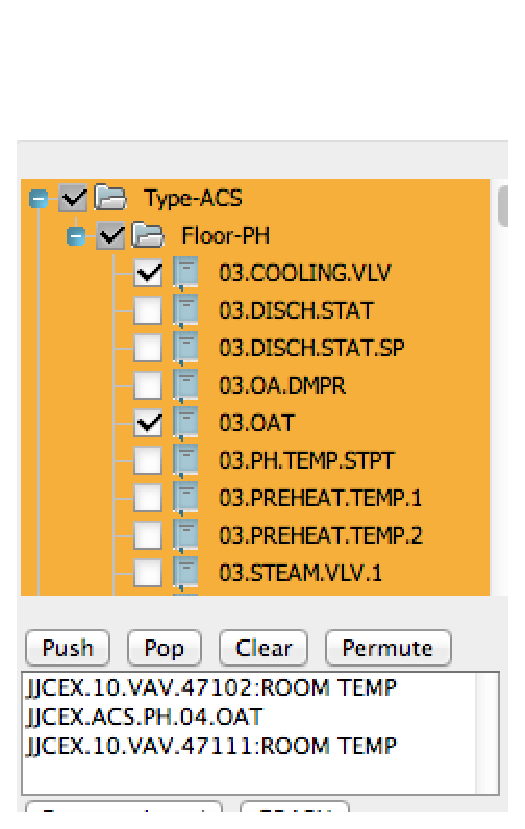
\includegraphics[scale=0.7]{fig1}


\subsection{The Selection Window}
The Selection Window will contain reference data that will be used during the analysis session. Users first choose what they want to include in the graphs
and/or the calculations. A mouse click on a plus sign on the left expands the type of sensor to location, which is expanded to  a mouse click on any of these expands the list to sensor name at the lowest level. To get these choice or choices into the selection window one clicks on the "PUSH" button below the window. 
By clicking in the box next to the sensor name, floor, or sensor category, users  choose one or several sensors, entire floors, or an entire categories.  
Once chosen, one must transfer their selections into the Selection Window, the first open window,
by pressing the "Push" button below the window. These steps  can be done multiple times,allowing the 
 hoosing of additional items.

Besides the "Push" button there are three others. 
To modify the order sequence of the listed sensors in the window, the button 'Permute' (see its use below) will swap the
selected item with the first item in the list. 'Clear' will clear all items and 'Pop' will remove the selected item.
 
If one just wants to graph the selected items against time, the "GRAPH" button below can be pressed. (The default is a time series (one of the choices to the left of the "GRAPH"botton; the other choices are described below.) The following windows allow more  other often complicated calculations to be done on the chosen items, such as only choosing some time periods,  doing computations on the sensor values, and restricting the sensor values to be graphed or included in calculations. 

{\bf Raw Data}\\
Below the selection box are two buttons : 'Filtered' and 'Unfiltered'. The purpose of these is to display all of part of raw data without any transformation except filtering: the filter box can be applied or not.
By default the entire selection is drawn. But choosing particular sensors is possible by selecting the ones to be drawn with Mouse Right Click, CTRL+Click and SHIFT+Click. 
This feature is very useful to compare data before and after transformation.

\subsection{The request box}
Another way to select sensors is to use a formula .
The request box contains a 'select' request to add a set of sensors instead of a manual selection.
\begin{lstlisting}
select(type = 'VAV", subtype = ['RM STPT DIAL','ROOM TEMP'], 
floor = 6, 
nexp = '47*',
pattern ='({i} - {i+1})',
cond='cmax(x,4)',
maxn = 20)
\end{lstlisting}
all parameters are optional.
\begin{itemize}
\item {\bf type} and {\bf subtype} are by default VAV and dial temp/room temp but can be anything
\item {\bf nexp} is a regular expression to filter out room numbers
\item {\bf pattern} is the type of operation, or expression, applied on a sensor 'i' . For instance {i} - {i+1} computes the difference between sensor i and  sensor i+1. Can be any arithmetic operation.
\item {\bf cond} : is a condition to be applied on the expression. Can be any Python function.
\item {\bf maxn} :is the max number of sensors to be displayed.
\end{itemize}



\subsection{The filter box}
Right under the selection stack we have the filter box.  
 The purpose of this box is to keep only those parts of the sensor or time line that the user wants  to be kept. 
 For example one can choose to only keep month 6 (June) or sensor values greater than a value  any expression composed of sensor values. 
For the purposes of filtering the rows (items)  in the Selection Box are implicitly indexed (0,1,2 etc.).
The index references are used during the filtering and the formatting phases.
The user writes expressions in the form of Python lambda functions in 'x' to filter out input data.
The filters are separated by ';' followed by a return. Each line matches
with the corresponding sensor from the Selection Stack, starting with
the time axis. That is the first line is used to filter the time axis, then line two for the first 
sensor listed on the stack, followed by sensor 2 , etc.

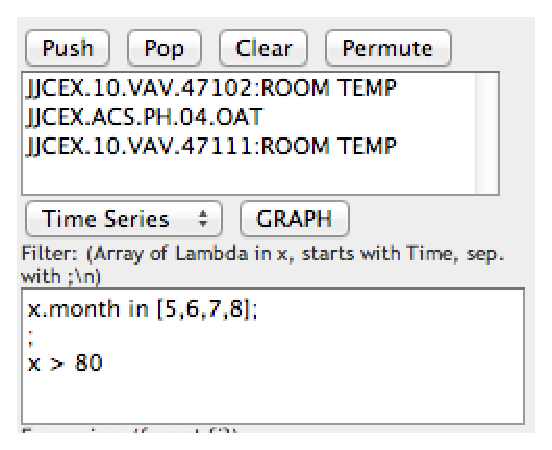
\includegraphics[clip,scale=0.7]{fig2}

In this example we want data for which the observation month is either 5,6,7 or 8. There
is no constraint on sensor 1, and sensor 2 must have values greater
than 80.


\subsubsection{The time axis filter}

More on filtering of the time. Time can make use of built-in Python functions which the following members are defined:

\begin{lstlisting}
x.year, x.month, x.day, x.hour, x.minute
\end{lstlisting}
Year is four digits, month is numeric, day is numeric 1 (sunday) through 7, hour is a 24 hour clock

Also:

\begin{lstlisting}
x.weekday(), x.replace()
\end{lstlisting}


One can even do comparisons  with a datetime object:

\begin{lstlisting}
x >= datetime(2013,2,1)
\end{lstlisting}


The complete documentation is available at :

\url{https://docs.python.org/2/library/datetime.html#datetime-objects}


\subsubsection{lambda x}

Almost all the sensors are represented as float 64 values, thus filters
will apply to Python floats. Boolean expression and math functions
are allowed, so it is possible to build complex queries, but sub function
definitions are not authorized. Math functions must be prefixed by
'math.' . Example :

\begin{lstlisting}
math.log(x) > 2 and math.sin(x) == math.pi;
\end{lstlisting}


More on Python expressions:

\url{https://docs.python.org/2/reference/expressions.html}

More on Python math module:

\url{https://docs.python.org/2/library/math.html}

\subsection{The expression boxes}
There is two expression boxes: one for graphing of data, and the other
for learning. The first, under the filter text field is used for graphing. 
It allows additional to the chosen sensors  expressions to be part of the graph
output. It is in fact like a Python string format expression,
but it is destined to be evaluated by the Python interpreter within
the context of the analysis: Every input is represented by a format
field within brackets: \{0\},\{1\}, etc.

\includegraphics[bb=0bp 0bp 249bp 105bp,clip]{fig3}


Behind these templates are Pandas objects, more precisely Pandas columns.
One has to see the output as a table where every column represents
a particular sensor (plus the time). What is evaluated prior to graph
is in fact a formatted expression. Basic arithmetics and special functions
are allowed, as well as basic boolean expressions (for which we will
prefer using the filter box because the syntax is much lighter).
\begin{itemize}
\item Reordering the output is then permitted : 
\begin{lstlisting}
{1};{0};{2}
\end{lstlisting}
 will display sensor 2, sensor 1 then sensor 3. This will be useful
during the forecast/training phase. Note : counting must starts at
0 and increments by 1.
\item Basic arithmetic:
\begin{lstlisting}
{1} - {0}; abs({1} - {0}); {1} - {0}/{1}*200
\end{lstlisting}

\item Basic Pandas built-ins (only those that returns a set) :
\begin{lstlisting}
{0}.diff(); {0}.pct_change();{0}.cumsum()
\end{lstlisting}

\item Special 'apply' function that allows math or lambda expressions:
\begin{lstlisting}
{0}.apply(math.sin); {0}.apply(lambda x : x if x <= 0 else math.log(x))
\end{lstlisting}

\item Special field '\{t\}' to access time axis: \{t\} represents a datetime
object
\begin{lstlisting}
{t}.hour%4
{t}.weekday()
\end{lstlisting}

\end{itemize}
The complete Pandas documentation on basic functions and expressions
is available here:

\url{http://pandas.pydata.org/pandas-docs/stable/basics.html#function-application}


\subsection{Graph Types}

Several graph types can be created. The following menu gives the possible
choices:

\includegraphics[clip,scale=0.7]{graph}

Data will be filtered out according to the filter box and several
graphs will be created following the template defined in the format
box.
\begin{itemize}
\item Time Series: Y's are the data, X is the time.
\item Moving Std: That will compute, for every data, the MA plus +/- 2 standard
deviations computed on a rolling period of 20 ticks (20 {*} 15 minutes).
It shows trend and values which are outside the STD envelope are likely
to be 'abnormal'.
\item XY : X axis is the first entry corresponding to the forma, Y's are
the next ones. By default X is going to be the element on top of the
stack. But it is possible to graph more complex expressions; for instance
\{2\}-\{1\},\{0\} in the format box will display (sensor 2 - sensor
1) in X and (sensor 0) in Y. XY values are sorted and unique.
\item Correl: Shows a rolling windows (20 elements) of cross correlations
between the first set of values compared to the others. 
\item Frequencies: Show an histogram of the value distribution, only for
the first element (for readability reasons)
\end{itemize}
All this types are compatible with filters and formats detailed above.
Note:In the latest version we added the possibility to display raw/input data, filtered or unfiltered, along computed expressions and machine learning statuses.

\section{Persistence}

The lab allows some basic persistence, it is possible to save/load
a context under a given name. The context consists in :
\begin{itemize}
\item sensor list
\item graph type
\item filter box and expression boxes
\item MAW and training size 
\item Machine type and learned set (if it exists)
\end{itemize}
To create a new context, simply type a name in the field :

\includegraphics[clip,scale=0.7]{p}

The new name is then added to the menu and can be loaded.

Training a new set will automatically save it, and if a name is not
provided then it will be saved under generic name 'tmp'. 

Context are stored on the server so every user can see them and thus
share their own sets.

Deleting a set is not possible for now and must be manually done by
the developers.


\section{Machine Learning}

BPL Research offers some machine learning features: from a given set
of data a machine can be trained and forecasts a specific output.

Machine input and output are defined the same way as graphs: Filters
are applied to the selected stack and an expression is eventually
computed. 

From there, 'Learn' button will start training. The reference output
is the first value defined in the Expression Box (by default it is
the top sensor on the stack) at T + 1 tick.

Inputs are the other values at T. Learning results are shown as a
graph comparing training values to forecast.

Training parameters are :
\begin{itemize}
\item MAW : moving average period (in ticks). A training/forecast can be
performed on moving average data instead of raw data. A MAW of 1 means
no moving average.
\item Train size: size of training set as a percentage of the input set.
The training set is uniformely sampled from the data set.
\item Machine type: as of today : SVM with Poly kernel, Gaussian multinomial, Logistic Regression and SVM Laplace  kernel.
\end{itemize}
Machine learning is entirely based on the Python Sci Kit libraries,
and adding new models can be done easily. More information on SciKit
:

\url{http://scikit-learn.org/stable/index.html}

So far, we have noticed that the best regressor seems to be SVM.

After training ('Learn' button), the trained set is saved as part
of the selected configuration and it's then possible to run it against
a different set of parameters, by modifying the sensor stack or the
expression box. Beware of the fact that the number of input must be
the same. 

\section{Advanced Features: Python plugins}
Users can upload their own python code and run it through the Expression box. A sandbox environment is under development as of today. But simple functions can yet be written.
Any python file can be uploaded and dynamically imported with buttons 'Choose File' and 'Upload'.
As the sandbox is not created yet, one must be very careful using this feature because it can lead to a server crash. 
The plugin python code is uploaded in the expression box running context and therefore the data model is accessible to new functions. Here the data model is based on Pandas. 
Plugins are exported in the application boxes through the namespace 'P'.
\subsection{Apply method}
In this application, selected datas are taken from a local DB and turned into Pandas data frames, on which the Filter and Expression are applied.
The simplest way to add python code is through the Pandas 'apply' method that calls a function on every row/column of a Pandas table. We have seen in 1.5 how to run lambda functions on the data, now we can extend this to regular python functions.
For example an expression such as: 
\begin{lstlisting}
 pdata.apply(f, axis=1)
\end{lstlisting}
will call the function 'f' on the entire data frame, f taking a row in argument:
\begin{lstlisting}
def f (row):
	return row[1] + row[2] etc.
\end{lstlisting}
Here, every index of the argument represents a data in the order of the selection.
\subsection{Generic call}
Furthermore, a generic data frame can be displayed if it respects the format of the application.
It is then possible to dig directly into the database and construct whatever data frame to be displayed. The constraint is such code must return a Pandas data frame with a datetime index. Then the dataset can be graphed with all the existing options or used as a learning set.
Functions used by the application to retrieve sensor data and training features can be reused as well.
\begin{lstlisting}
def run():
    rng = pandas.date_range('1/1/2011', periods=72, freq='H')
    return pandas.Series(numpy.random.randn(len(rng)), index=rng)
\end{lstlisting}
Calling 'P.run()' will graph a random data set.


\section{Notes on code}

The entire application is based on Python, the front end being HTML
and JavaScript, and the framework is based on Django. 

Source is available from CVS : :pserver:eric@rscript.cisdd.org:/home/eric/cvsrepo
\end{document}
